%%%%%%%%%%%%%%%%%%%%%%%%%%%%%%
% NOTE. It takes a good minute to typeset
%%%%%%%%%%%%%%%%%%%%%%%%%%%%%%
\RequirePackage{luatex85}
\documentclass[tikz]{standalone}
\usepackage{expl3}
\ExplSyntaxOn
\cs_new_eq:NN \Repeat \prg_replicate:nn
\ExplSyntaxOff

\begin{document}
\Repeat{2}{
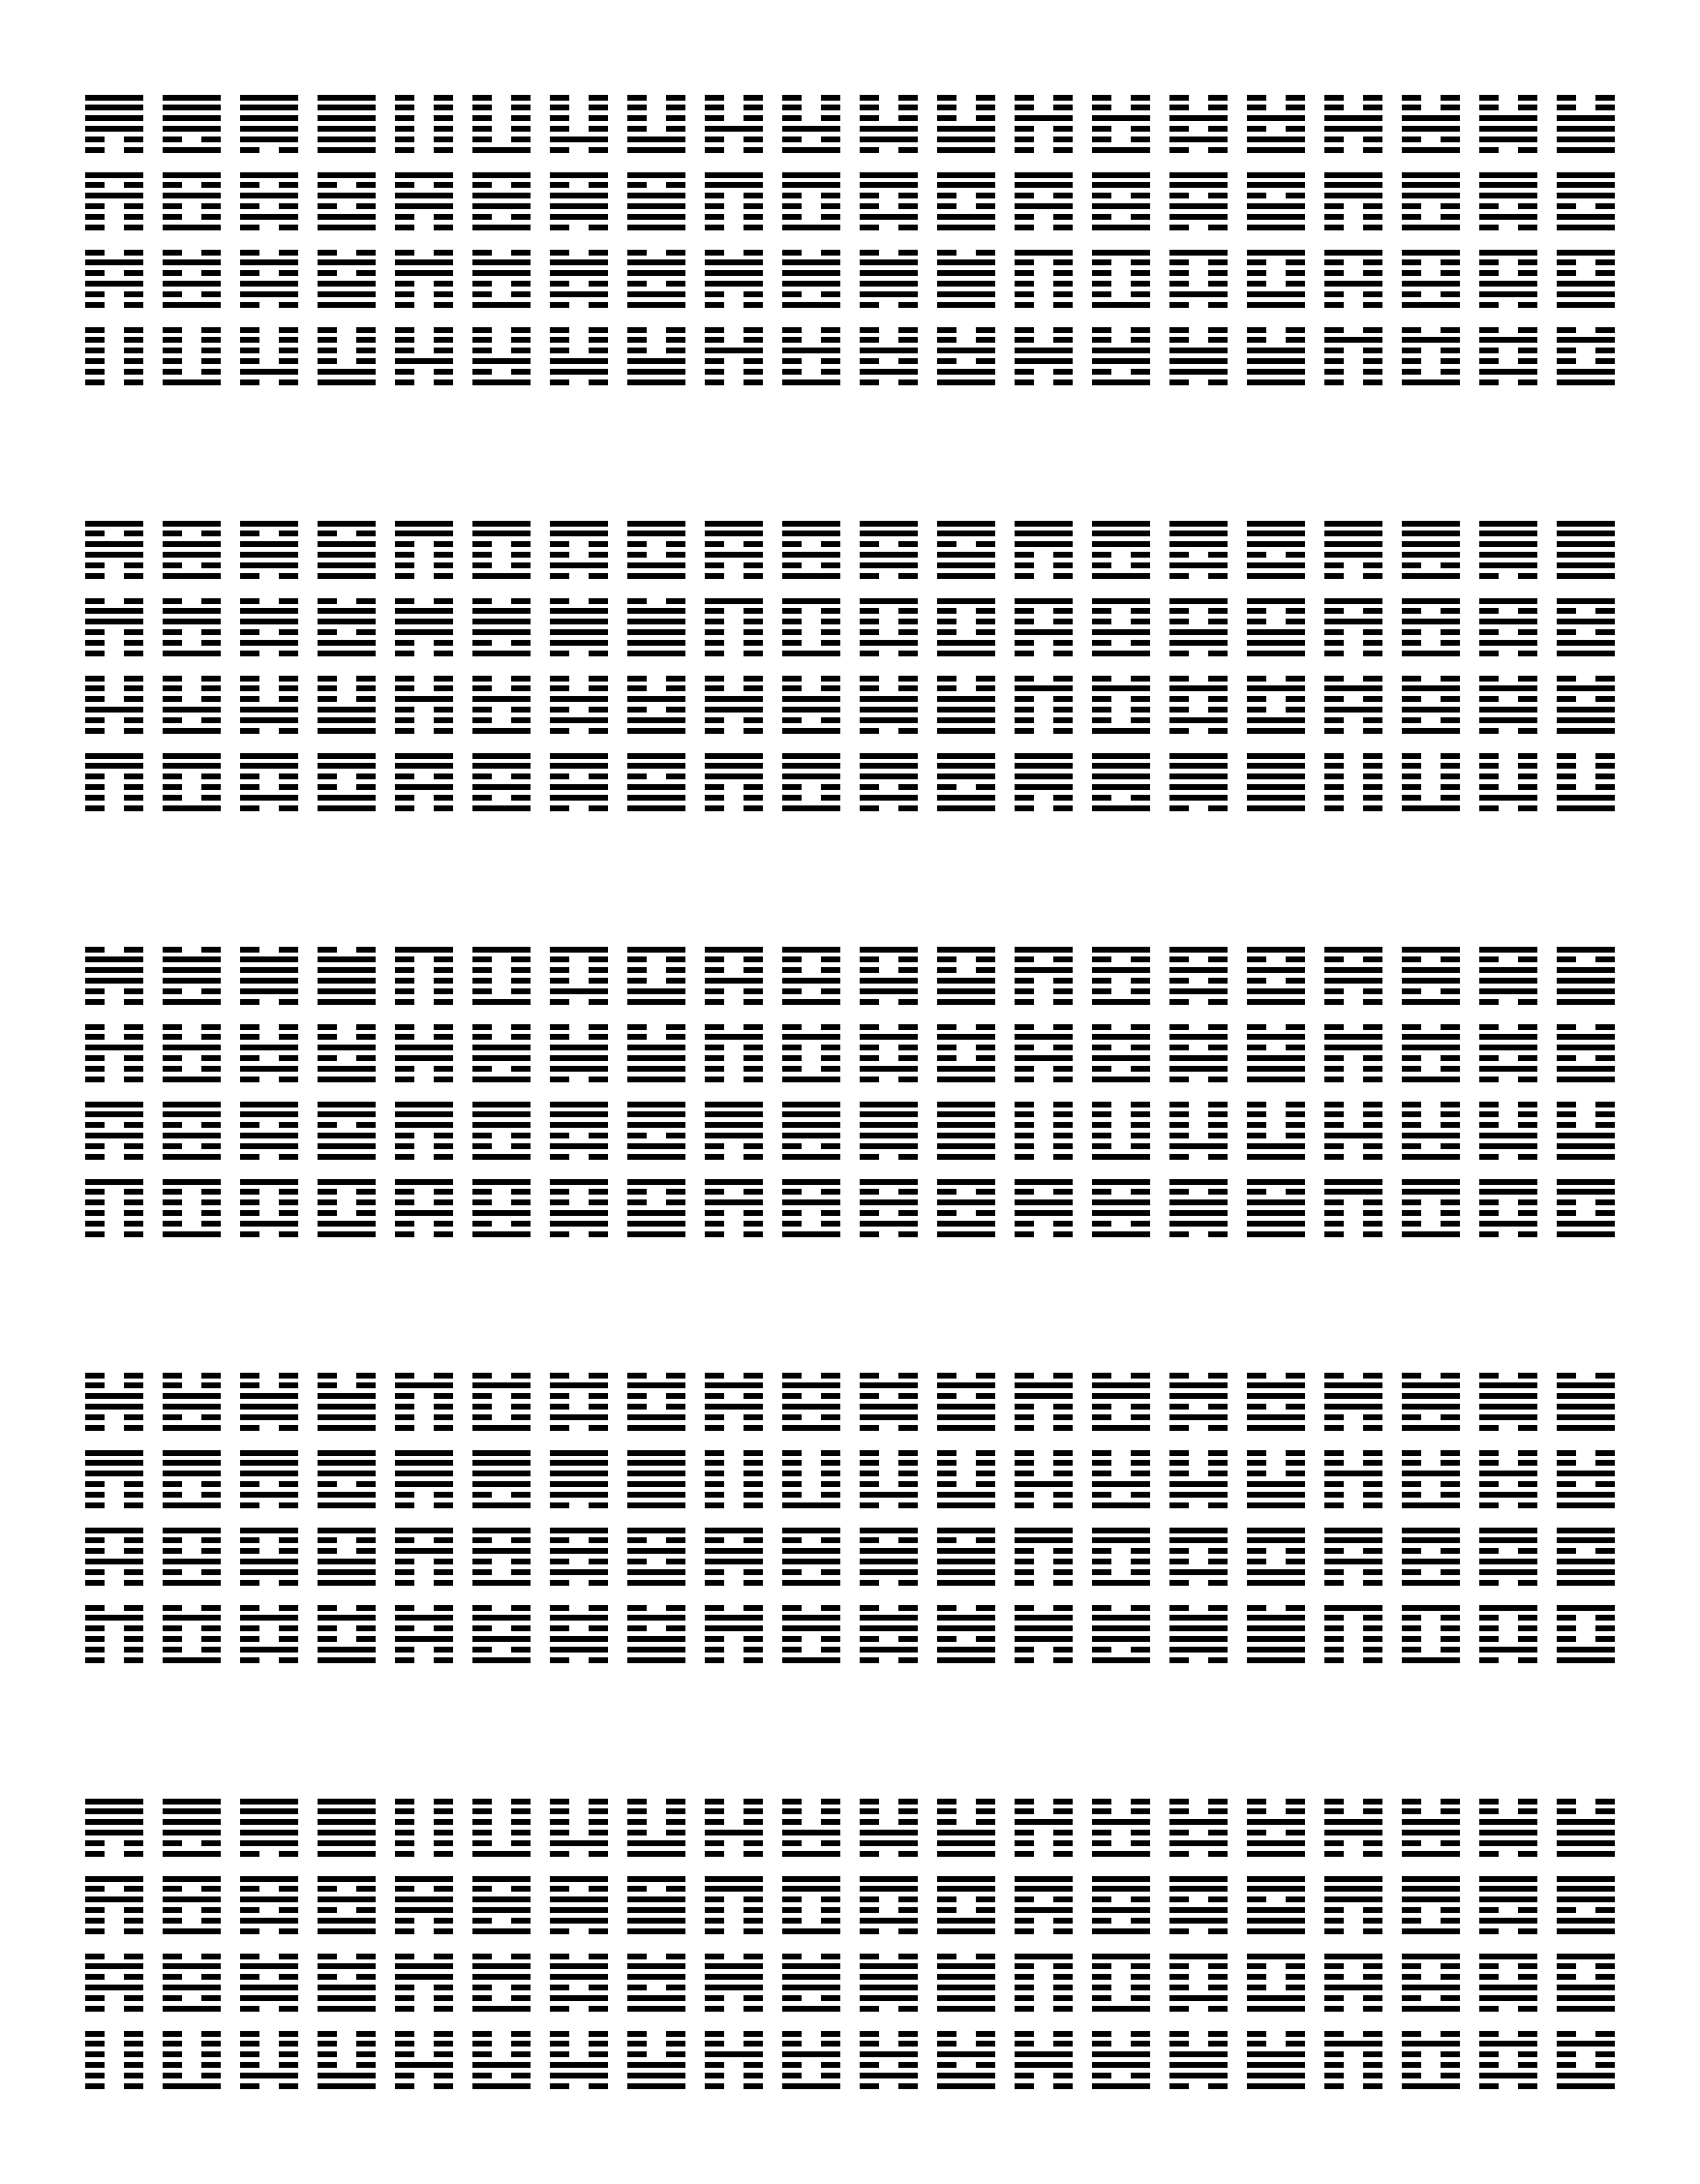
\begin{tikzpicture}
[line width=0.030in]
\clip (0,0) rectangle (8.5in,11in);
\foreach \sec in {0,...,4}{
\foreach \row in {0,...,3}{
\foreach \col in {0,...,19}{
\foreach \bar in {0,...,5}{
\draw ({0.300in+\col*0.400in},
{0.365in+\bar*0.054in+\row*0.400in+\sec*2.200in})
coordinate (xy);
\pgfmathtruncatemacro\val{
mod(floor(mod(\col+20*\row+80*\sec,64)/2^\bar),2)}
\ifnum\val=0
\draw (xy) -- ++(right:0.100in) ++(right:0.100in) -- ++(right:0.100in);
\else\draw (xy) -- ++(right:0.300in);\fi
}}}}
%\draw[step=0.1in, thin] (0,0) grid (8.5in,11in);
\end{tikzpicture}
}

\Repeat{2}{
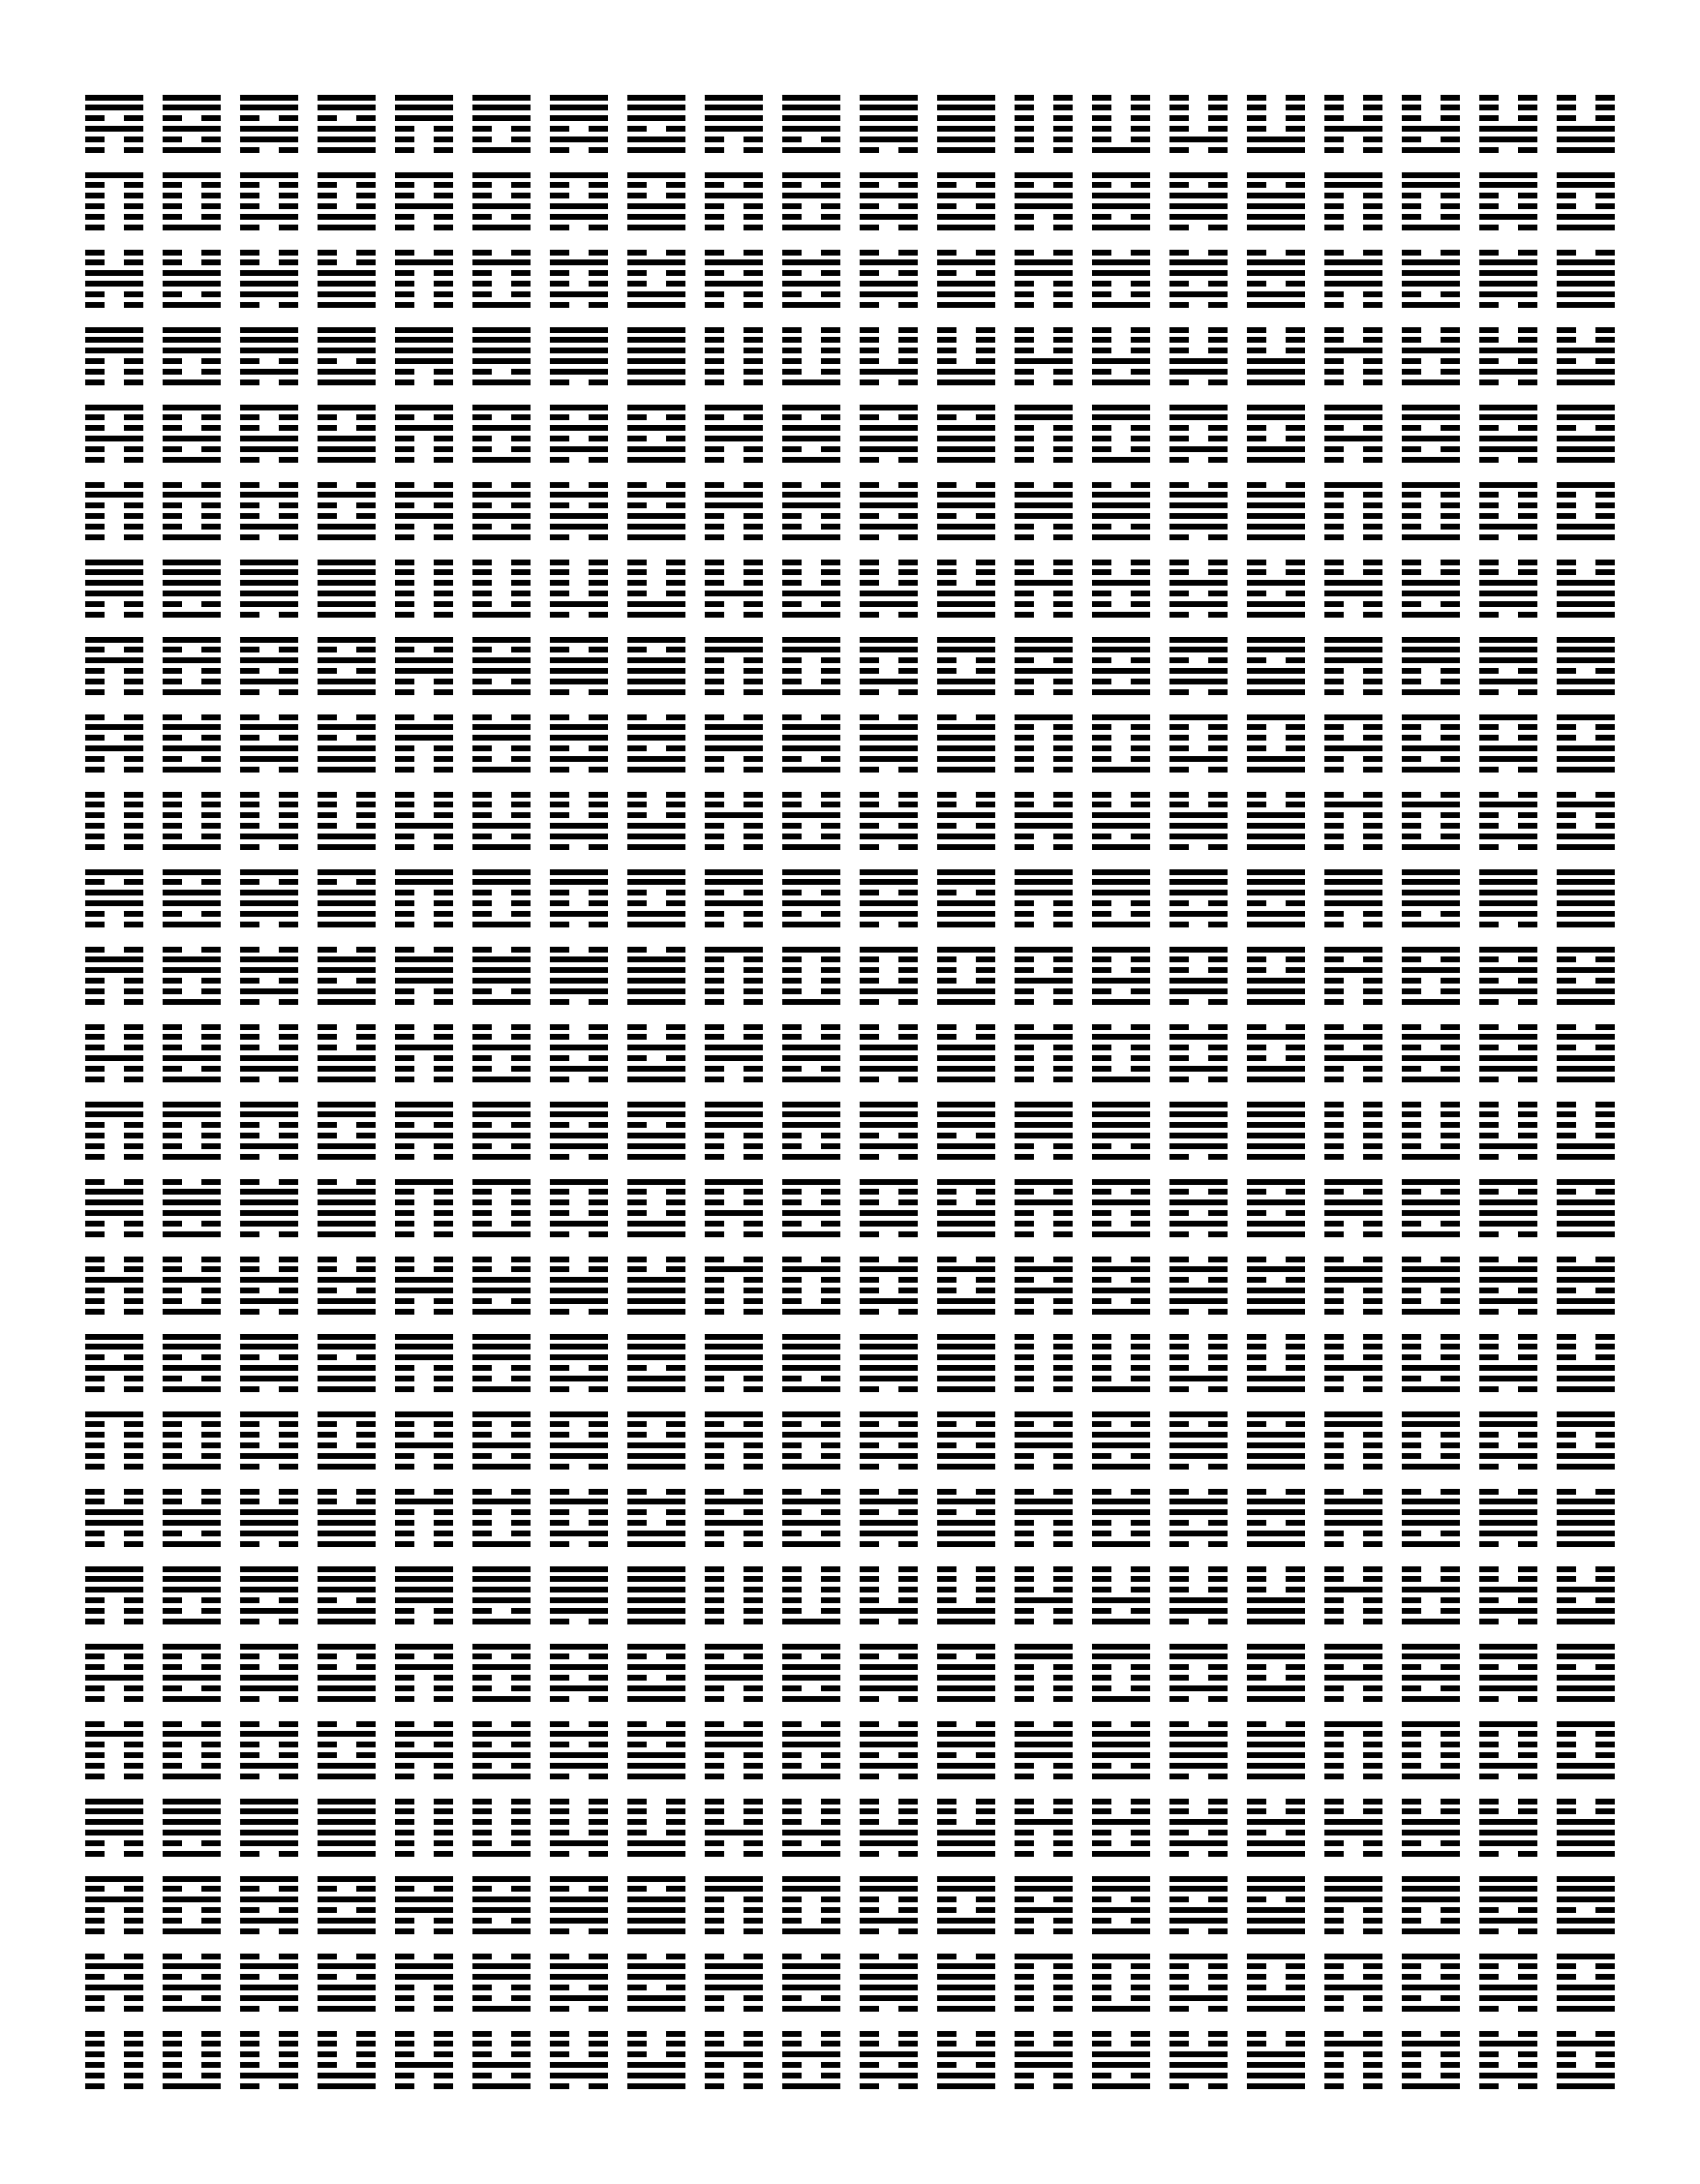
\begin{tikzpicture}
[line width=0.030in]
\clip (0,0) rectangle (8.5in,11in);
\foreach \sec in {0,...,0}{
\foreach \row in {0,...,25}{
\foreach \col in {0,...,19}{
\foreach \bar in {0,...,5}{
\draw ({0.300in+\col*0.400in},
{0.365in+\bar*0.054in+\row*0.400in+\sec*11.000in})
coordinate (xy);
\pgfmathtruncatemacro\val{
mod(floor(mod(\col+20*\row+520*\sec,64)/2^\bar),2)}
\ifnum\val=0
\draw (xy) -- ++(right:0.100in) ++(right:0.100in) -- ++(right:0.100in);
\else\draw (xy) -- ++(right:0.300in);\fi
}}}}
%\draw[step=0.1in, thin] (0,0) grid (8.5in,11in);
\end{tikzpicture}
}
\end{document}

%%%%%%%%%%%%%%%
% GENERATE TIKZ CODE
%%%%%%%%%%%%%%%
def tikzhexagrams(numsecs, numrows, numcols, 
		leftmargin, barlen, xsep,
		botmargin, barwidth, barsep, ysep):
	print("\\begin{tikzpicture}")
	print(f"[line width={barwidth:0.3f}in]")
	print("\\clip (0,0) rectangle (8.5in,11in);")
	print(f"\\foreach \\sec in \u007B0,...,{numsecs-1}\u007D\u007B")
	print(f"\\foreach \\row in \u007B0,...,{numrows-1}\u007D\u007B")
	print(f"\\foreach \\col in \u007B0,...,{numcols-1}\u007D\u007B")
	print("\\foreach \\bar in {0,...,5}{")
	print(f"\\draw (\u007B{leftmargin:0.3f}in", end="")
	print(f"+\\col*{xsep+barlen:0.3f}in\u007D,")
	print(f"\u007B{botmargin+0.5*barwidth:0.3f}in", end="")
	print(f"+\\bar*{barwidth+barsep:0.3f}in", end="")
	print(f"+\\row*{6*barwidth+5*barsep+ysep:0.3f}in", end="")
	print(f"+\\sec*{11/numsecs:0.3f}in\u007D)")
	print("coordinate (xy);")
	print("\\pgfmathtruncatemacro\\val{")
	print(f"mod(floor(mod(\\col+{numcols}*\\row", end="")
	print(f"+{numcols*numrows}*\\sec,64)/2^\\bar),2)\u007D")
	print("\\ifnum\\val=0")
	print(f"\\draw (xy) -- ++(right:{barlen/3:0.3f}in) ", end="")
	print(f"++(right:{barlen/3:0.3f}in) -- ++(right:{barlen/3:0.3f}in);")
	print(f"\\else\\draw (xy) -- ++(right:{barlen:0.3f}in);\\fi")
	print("}}}}")
	print("%\draw[step=0.1in, thin] (0,0) grid (8.5in,11in);")
	print("\\end{tikzpicture}")

tikzhexagrams(5, 4, 20,   0.3, 0.3, 0.1,   0.35, 0.03, 0.024, 0.1)
tikzhexagrams(1, 26, 20,   0.3, 0.3, 0.1,   0.35, 0.03, 0.024, 0.1)
#tikzhexagrams(5, 5, 21,   0.2, 0.3, 0.09,   0.2, 0.03 0.024, 0.075)
#tikzhexagrams(5, 5, 20,   0.3, 0.3, 0.1,   0.3, 0.02, 0.02, 0.125)